\documentclass[a4paper,11pt]{article}

\usepackage[french]{babel}
\usepackage[utf8]{inputenc}
\usepackage[left=2.5cm,top=2cm,right=2.5cm,nohead,nofoot]{geometry}
\usepackage{url}
\usepackage{graphicx}
\usepackage{hyperref}
\usepackage{listings}
\usepackage{amsmath}
\usepackage{amssymb}
\usepackage{color}
\usepackage{listings}
\usepackage{graphicx}
\usepackage{float}




\linespread{1.1}



\begin{document}

\begin{titlepage}
\begin{center}
\textbf{\textsc{UNIVERSIT\'E LIBRE DE BRUXELLES}}\\
%\textbf{\textsc{Faculté des Sciences}}\\
%\textbf{\textsc{Département d'Informatique}}
\vfill{}\vfill{}
\begin{center}{\Huge Projet : Logique Propositionnelle et Utilisation de l’Outil MiniSat}\end{center}{\Huge \par}
\begin{center}{\large Pierre Gérard, Antoine Carpentier}\end{center}{\Huge \par}
\vfill{}\vfill{} \vfill{}
\begin{flushleft}{\large \textbf{INFO-F-302 Informatique Fondamentale}}\hfill{Emmanuel FILIOT, Guillermo Pérez}\end{flushleft}{\large\par}
\vfill{}\vfill{}\enlargethispage{3cm}
\textbf{Année académique 2014~-~2015}
\end{center}
\end{titlepage}

%\begin{abstract}
%Ce rapport présente ...
%\end{abstract}


\tableofcontents

\pagebreak


\section{Q1}
Les contraintes sont les suivantes :
\begin{itemize}
  \item Contrainte d'existence : chaque examen se déroule dans au moins une salle et durant au moins une période de temps,
  \item Le nombre d'étudiant dans une salle ne peut pas dépasser sa capacité,
  \item Un étudiant ne peut pas avoir deux examens au même moment,
  \item Un professeur ne peut pas avoir deux examens au même moment,
  \item Un examen doit avoir au moins un professeur,
  \item Un examen doit avoir au moins un étudiant
  \item Chaque examen doit se dérouler une seule fois,
  \item Chaque examen doit se dérouler dans une seule salle,
  \item Dans une salle, il ne peut se déroule qu'un seul examen a la fois.
\end{itemize}


\section{Q2}
\subsection{Contrainte d'existence : chaque examen se déroule dans au moins une salle et durant au moins une période de temps}
\begin{displaymath}
	\forall x \in X, \exists s \in S, \exists t \in T : \mu(x) = (s,t) 
\end{displaymath}

\subsection {Le nombre d'étudiant dans une salle ne peut pas dépasser sa capacité}
\begin{displaymath}
\forall x \in X , \forall s \in S ,\forall e \in E, \forall t \in \{1,...,T\} : a(e) \mapsto \{x\} \wedge \mu(x) = (s,t) \wedge \sum a(e) \mapsto \{x\} \leq c(s)
\end{displaymath}	

\subsection {Un étudiant ne peut pas avoir deux examens au même moment}
\begin{displaymath}
\forall x_{1},x_{2} \in X, \forall s_{1},s_{2} \in S , \forall e \in E ,\forall t_{1}, t_{2} \in \{1,...,T\} :  a(e) \mapsto \{x_{1},x_{2}\}  \wedge \mu(x_{1}) = (s_{1},t_{1}) \wedge \mu(x_{2}) = (s_{2},t_{2}) \wedge t_{1} != t_{2} \wedge x_{1} != x_{2}
\end{displaymath}
\subsection {Un professeur ne peut pas avoir deux examens au même moment}
\begin{displaymath}
\forall x_{1},x_{2} \in X, \forall s_{1},s_{2} \in S , \forall p \in P ,\forall t_{1}, t_{2} \in \{1,...,T\} :  b(p) \mapsto \{x_{1},x_{2}\}  \wedge \mu(x_{1}) = (s_{1},t_{1}) \wedge \mu(x_{2}) = (s_{2},t_{2}) \wedge t_{1} != t_{2} \wedge x_{1} != x_{2}
\end{displaymath}
\subsection {Un examen doit avoir au moins un professeur}
\begin{displaymath}
\forall x \in X, \exists p \in P : b(p) \mapsto \{x\} 
\end{displaymath}
\subsection {Un examen doit avoir au moins un étudiant}
\begin{displaymath}
\forall x \in X, \exists e \in E : a(e) \mapsto \{x\}
\end{displaymath}
\subsection {Chaque examen doit se dérouler une seule fois}
\begin{displaymath}
\forall t_{1}, t_{2} \in \{1,...,T\},\forall s_{1},s_{2} \in S, \nexists x \in X : t_{1} != t_{2} \wedge \mu(x) = (s_{1},t_{1}) \wedge \mu(x) = (s_{2},t_{2})
\end{displaymath}
\subsection {Chaque examen doit se dérouler dans une seule salle}
\begin{displaymath}
\forall t_{1}, t_{2} \in \{1,...,T\},\forall s_{1},s_{2} \in S, \nexists x \in X : s_{1} != s_{2} \wedge \mu(x) = (s_{1},t_{1}) \wedge \mu(x) = (s_{2},t_{2})
\end{displaymath}	
\subsection {Dans une salle, il ne peut se dérouler qu'un seul examen a la fois}
\begin{displaymath}
\forall t_{1}, t_{2} \in \{1,...,T\},\forall x_{1},x_{2} \in X, \nexists s \in S : t_{1} = t_{2} \wedge x_{1} != x_{2} \wedge \mu(x_{1}) = (s,t_{1}) \wedge \mu(x_{2}) = (s,t_{2})
\end{displaymath}	

\section{Q3}
Pour construire la formule en FNC, nous avons besoins de définir de nouvelle variable.
\begin{itemize}
    \item \(E\) est le nombre d'étudiants
    \item \(P\) est le nombre de professeurs
    \item \(X\) est le nombre d'examens
    \item \(S\) est le nombre de salles
    \item \(T\) est le nombre de périodes de temps
	\item \( A_{e,x}\) telle que l'étudiant e passe l'examen x,
	\item \(B_{p,x}\) telle que le professeur p donne l'examen x ,
	\item \(C_{s,i}\) telle que la salle s a la capacité d'accueillir i étudiants,
	\item \(N_{x}\) telle que la fonction N donne le nombre d'étudiant qui passe l'examen x.
\end{itemize}


\subsection{Ensemble de FNC}
\subsubsection{(p1)}
Contrainte d'existence : chaque examen se déroule dans au moins une salle et durant au moins une période de temps
\begin{displaymath}
	\bigwedge\limits_{x=1}^{X}\bigvee\limits_{s=1}^{S}\bigvee\limits_{t=1}^{T} M_{s,x,t}
\end{displaymath}


\subsubsection{(p2)}
Le nombre d'étudiant dans une salle ne peut pas dépasser sa capacité
\begin{displaymath}
	\bigwedge\limits_{t=1}^{T}\bigwedge\limits_{x=1}^{X}\bigwedge\limits_{\substack{s=1 \\ \neg C_{s,N_{x}}}}^{S}  \neg M_{x,s,t}
\end{displaymath}

\subsubsection{(p3)}
Un étudiant ne peut pas avoir deux examens au même moment
\begin{displaymath}
\bigwedge\limits_{e=1}^{E}\bigwedge\limits_{t=1}^{T}\bigwedge\limits_{s_{1}=1}^{S}\bigwedge\limits_{s_{2}=1}^{S}\bigwedge\limits_{\substack{x1=1 \\ A_{e,x_{1}}}}^{X}\bigwedge\limits_{\substack{x_{2}=x_{1}+1 \\ A_{e,x_{2}}}}^{X} \neg M_{x_{1}, s_{1}, t} \vee \neg M_{x_{2}, s_{2}, t}
\end{displaymath}

\subsubsection{(p4)}
Un professeur ne peut pas avoir deux examens au même moment
\begin{displaymath}
\bigwedge\limits_{p=1}^{P}\bigwedge\limits_{t=1}^{T}\bigwedge\limits_{s_{1}=1}^{S}\bigwedge\limits_{s_{2}=1}^{S}\bigwedge\limits_{\substack{x_{1}=1 \\ B_{p,x_{1}}}}^{X}\bigwedge\limits_{\substack{x_{2}=x_{1}+1 \\ B_{p,x_{2}}}}^{X} \neg M_{x_{1}, s_{1}, t} \vee \neg M_{x_{2}, s_{2}, t}
\end{displaymath}

\subsubsection{(p5)}
Un examen doit avoir au moins un professeur
\begin{displaymath}
\bigwedge\limits_{x=1}^{X}\bigvee\limits_{s=1}^{S}\bigvee\limits_{t=1}^{T}\bigvee\limits_{\substack{p=1 \\ B_{p,x}}}^{P} M_{x, s, t}
\end{displaymath}

\subsubsection{(p6)}
Un examen doit avoir au moins un étudiant
\begin{displaymath}
\bigwedge\limits_{x=1}^{X}\bigvee\limits_{s=1}^{S}\bigvee\limits_{t=1}^{T}\bigvee\limits_{\substack{e=1 \\ A_{e,x}}}^{E} M_{x, s, t}
\end{displaymath}

\subsubsection{(p7)}
Chaque examen doit se dérouler une seule fois
\begin{displaymath}
\bigwedge\limits_{x=1}^{X}\bigwedge\limits_{s=1}^{S}\bigwedge\limits_{t_{1}=1}^{T}\bigwedge\limits_{t_{2}=t_{1}+1}^{T} \neg M_{x, s, t_{1}} \vee \neg M_{x, s, t_{2}}
\end{displaymath}

\subsubsection{(p8)}
Chaque examen doit se dérouler dans une seule salle
\begin{displaymath}
\bigwedge\limits_{x=1}^{X}\bigwedge\limits_{t=1}^{T}\bigwedge\limits_{s_{1}=1}^{S}\bigwedge\limits_{s_{2}=t1+1}^{S} \neg M_{x, s_{1}, t} \vee \neg M_{x, s_{2}, t}
\end{displaymath}

\subsubsection{(p9)}
Dans une salle, il ne peut se déroule qu'un seul examen a la fois.
\begin{displaymath}
\bigwedge\limits_{s=1}^{S}\bigwedge\limits_{t=1}^{T}\bigwedge\limits_{x_{1}=1}^{X}\bigwedge\limits_{x_{2}=t1+1}^{X} \neg M_{x_{1}, s, t} \vee \neg M_{x_{2}, s, t}
\end{displaymath}


\subsection{FNC final}
La forme normal conjonctive de la formule est:
\begin{displaymath}
\Phi_{I} = p1 \wedge p2 \wedge p3 \wedge p4 \wedge p5 \wedge p6 \wedge p7 \wedge p8 \wedge p9
\end{displaymath}

\section{Q4}
\subsection{Tester l'implémentation}
Pour tester l'implémentation, utilisez le script bash disponible de la manière suivante :
\begin{lstlisting}
$ sh TestMe.sh	
\end{lstlisting}
Ce script va faire le build, lire les fichiers, et exécuter mini-sate.

\subsection{Parser}
Pour le parser, nous avons décidé de ne pas utiliser l'ensemble du code du parser fournit. Nous avons donc seulement gardé la classe ShedSpec en créant nous même la structure de donnée nécessaire pour son constructeur.

\subsection{Implémentation}

% TODO

\subsection{Exemple de résultat}
Nous avons créé une liste d'input possible pour cette question. Voici quelque exemple
\subsubsection{Construction d'un horaire possible}
Input fournis avec l'énoncé.
\begin{lstlisting}[
    basicstyle=\tiny, %or \small or \footnotesize etc.
]
$ ./projq4.out "4 ;3 ;10 ;30 ;100 ;100 ;2 ;4 ;1; 1; 1 ;1 ;1 ;1 ;1 ;1 ;1 ;1 ;1 ;1 ;1 ;1 ;1 ;1 ;1 ;1 ;1 ;1
 ;1 ;1 ;1 ;1 ;1 ;1 ;1 ;1 ;1 ;1 ;2 ;2 ;2 ;2 ;2 ;2 ;2 ;2 ;2 ;2 ;2 ;2 ;2 ;2 ;2 ;2 ;2 ;2 ;2 ;2 ;2 ;2 ;2 ;2 
 ;2 ;2 ;2 ;2 ;2 ;2 ;3,4 ;3,4 ;3,4 ;3,4 ;3,4 ;3,4 ;3,4 ;3,4 ;3,4 ;3,4 ;3,4 ;3,4 ;3,4 ;3,4 ;3,4 ;3,4 
 ;3,4 ;3,4 ;3,4 ;3,4 ;3,4 ;3,4 ;3,4 ;3,4 ;3,4 ;3,4 ;3,4 ;3,4 ;3,4 ;3,4 ;3,4 ;3,4 ;3,4 ;3,4 ;3,4 ;3,4 
 ;3,4 ;3,4 ;3,4 ;3,4 ;1,3 ;2,4;
---------------------------------------- Result ----------------------------------------
T = 4
|S| = 3
c(s1) = 10
c(s2) = 30
c(s3) = 100
|E| = 100
|P| = 2
|X| = 4
a(e1) = { 1 }
[...]
a(e30) = { 1 }
[...]
a(e60) = { 2 }
a(e61) = { 3 4 }
[...]
a(e99) = { 3 4 }
a(e100) = { 3 4 }
b(p1) = { 1 3 }
b(p2) = { 2 4 }
==================================[MINISAT]===================================
| Conflicts |     ORIGINAL     |              LEARNT              | Progress |
|           | Clauses Literals |   Limit Clauses Literals  Lit/Cl |          |
==============================================================================
|         0 |     260     3528 |      86       0        0     nan |  0.000 % |
==============================================================================
Success, the problem has been solve under those constraints !
Examen 1 dans la salle 2 au temps 1
Examen 2 dans la salle 2 au temps 2
Examen 3 dans la salle 3 au temps 2
Examen 4 dans la salle 3 au temps 1

OUTPUT : 2,1;2,2;3,2;3,1;
\end{lstlisting}

\subsubsection{Construction d'un horaire impossible}
Input créé de tel manière qu'il n'y ait pas moyen de construire un horaire.
\begin{lstlisting}[
    basicstyle=\tiny, %or \small or \footnotesize etc.
]
$ ./projq4.out "1 ;3 ;1 ;10 ;50 ;2 ;2 ;2 ;1,2 ;1 ;1 ;2 ;"
---------------------------------------- Result ----------------------------------------
T = 1
|S| = 3
c(s1) = 1
c(s2) = 10
c(s3) = 50
|E| = 2
|P| = 2
|X| = 2
a(e1) = { 1 2 }
a(e2) = { 1 }
b(p1) = { 1 }
b(p2) = { 2 }
==================================[MINISAT]===================================
| Conflicts |     ORIGINAL     |              LEARNT              | Progress |
|           | Clauses Literals |   Limit Clauses Literals  Lit/Cl |          |
==============================================================================
|         0 |      18       53 |       6       0        0     nan |  0.000 % |
==============================================================================
Uh .. The problem could not be solve under those constraints

OUTPUT : 0
\end{lstlisting}

\section{Q5}
Pour construire la formule en FNC, nous avons besoins de définir une nouvelle variable :  
\begin{itemize}
	\item \( D_{x}\) qui donne la durée de l'examen x.
\end{itemize}

\subsection{Modification de contrainte}

\subsubsection{(p3)}
Un étudiant ne peut pas avoir deux examens au même moment
\begin{displaymath}
\bigwedge\limits_{e=1}^{E}\bigwedge\limits_{t1=1}^{T}\bigwedge\limits_{\substack{t2=1 \\ t1 <= t2 + D(x2)-1 \wedge t1 + D(x1)-1 >= t2}}^{S}\bigwedge\limits_{s=1}^{S}\bigwedge\limits_{\substack{x1=1 \\ A_{e,x1}}}^{X}\bigwedge\limits_{\substack{x2=x1+1 \\ A_{e,x2}}}^{X} \neg M_{x1, s1, t} \vee \neg M_{x2, s2, t}
\end{displaymath}

\subsubsection{(p4)}
Un professeur ne peut pas avoir deux examens au même moment
\begin{displaymath}
\bigwedge\limits_{p=1}^{P}\bigwedge\limits_{t1=1}^{T}\bigwedge\limits_{\substack{t2=1 \\ t1 <= t2 + D(x2)-1 \wedge t1 + D(x1)-1 >= t2}}^{S}\bigwedge\limits_{s=1}^{S}\bigwedge\limits_{\substack{x1=1 \\ B_{p,x1}}}^{X}\bigwedge\limits_{\substack{x2=x1+1 \\ B_{p,x2}}}^{X} \neg M_{x1, s1, t} \vee \neg M_{x2, s2, t}
\end{displaymath}


\subsection{Nouvelle contrainte}
Les nouvelles contraintes sont :
\subsubsection{Chaque examen doit avoir un nombre de période de de temps égal à sa durée et ses périodes de temps doivent être continues}

(p10)
\begin{displaymath}
\bigwedge\limits_{x=1}^{X}\bigwedge\limits_{\substack{x2=1 \\ x1 != x2}}^{X}\bigwedge\limits_{s=1}^{S}\bigwedge\limits_{t1=1}^{T}\bigvee\limits_{\substack{t2=0 \\ t1 <= t2 + D(x2)-1 \wedge t1 + D(x1)-1 >= t2}}^{T} \neg M_{x, s, t1} \vee \neg M_{x2, s2, t2}
\end{displaymath}

\subsection{FNC}

\begin{displaymath}
	\Phi_{D} = p1 \wedge p2 \wedge p3 \wedge p4 \wedge p5 \wedge p6 \wedge p8 \wedge p9 \wedge p10
\end{displaymath}

\subsection{Implémentation}

\subsection{Exemple de résultats}

\section{Q6}

\section{Q7}

\section{Q8}

\section{Q9}

\section{Q10}

LES ETUDIANTS VEULENT BOUFFER LE TEMPS DE MIDI !!!!!!!!!
durée max d'un examen
le week end
overbooking sur les salles
certain examen dans certain salle (salle info)


\section{Q11}
Un problème NP-complet est NP-dur par définition. En effet, comme montré sur l'image suivante NP-complet est un sous-ensemble de NP-dur et de NP.
\begin{figure}[H]
  \centering
  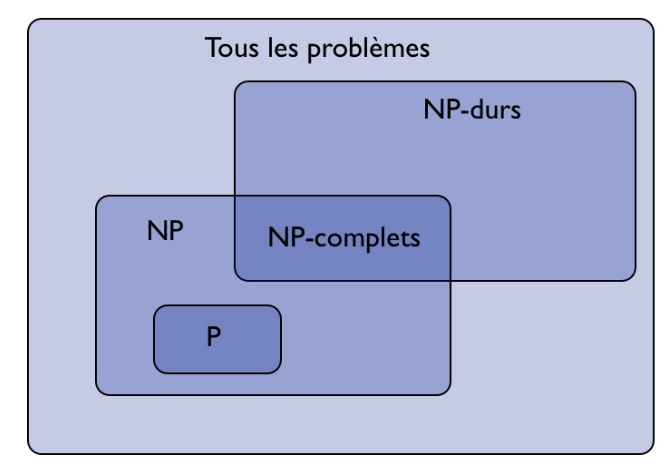
\includegraphics[scale=0.4]{images/q11-p-np-nphardcomplete.png}
  \caption{\label{} P, NP, NP-complet et NP-dur}
\end{figure}
D'après le \textit{Théorème de Cook}, SAT est un problème NP complet. Donc SAT est aussi un problème NP-Dur.

Lors de ce projet nous avons réduit le problème d'emploi de temps en un problème SAT.

On peut donc déduire que le problème d'emploi du temps est un problème NP-dur.

%Un problème est NP-complet est NP-dur si il peut se ramener sous la forme d'un autre problème NP-complet. Si un problème peut se mettre en forme normal conjonctive et satisfaisable, il est SAT. Notre problème possède au moins 3 clauses, en effet TODO . Il est donc 3-SAT et donc il est aussi NP-complet donc on peut déduire que notre problème est NP-complet ou NP-dur.
\end{document}

